% !TEX root = ../Tesis.tex
\chapter{Evaluación de desempeño} 
\label{cap:evaluación de desempeño} 

En este capítulo se muestran los resultados que se obtuvieron en las métricas mencionadas. Para los modelos sin DWT se muestra únicamente el RMSE, MAPE y DS de la predicción del conjunto de prueba contra los precios reales. Para los restantes se pinta un desglose de cada medida por cada componente y la reconstrucción total del pronóstico del conjunto de pruebas.

\section{Predicción Estándar}

\begin{longtable}{lccc}
\textbf{NARNN | muestreo aleatorio} & \textbf{RMSE} & \textbf{MAPE (\%)} & \textbf{DS (\%)} \\
\textbf{Predicción de c\_prueba} & 1.014 & 7.21322 & 63.7097 \\
\textbf{DWT-NARNN | muestreo aleatorio} & & & \\
\textbf{Reconstrucción de c\_prueba} & 1.0769 & 7.397269 & 65.1515 \\
\textbf{Componente A5} & 1.0502 & 7.186337 & 62.8788 \\
\textbf{Componente D5} & 0.0000 & 133.993170 & 68.9394 \\
\textbf{Componente D4} & 0.0000 & 109.625883 & 62.8788 \\
\textbf{Componente D3} & 0.0000 & 102.676865 & 74.2424 \\
\textbf{Componente D2} & 0.0000 & 154.036830 & 70.4545 \\
\textbf{Componente D1} & 0.1402 & 315.594656 & 58.3333 \\

\textbf{LSTM | muestreo aleatorio} &  &  &  \\
\textbf{Predicción de c\_prueba} & 0.8335 & 6.015341 & 62.0968 \\
\textbf{DWT-LSTM | muestreo aleatorio} &  &  &  \\
\textbf{Reconstrucción de c\_prueba} & 0.8689 & 5.887960 & 68.1818 \\
\textbf{Componente A5} & 0.8488 & 5.699098 & 58.3333 \\
\textbf{Componente D5} & 0.0000 & 62.915075 & 81.0606 \\
\textbf{Componente D4} & 0.0000 & 95.984062 & 84.8485 \\
\textbf{Componente D3} & 0.0000 & 68.514078 & 79.5455 \\
\textbf{Componente D2} & 0.0000 & 69.674597 & 78.7879 \\
\textbf{Componente D1} & 0.1195 & 1924.748875 & 81.8182 \\

\textbf{GRU | muestreo aleatorio} &  &  &  \\
\textbf{Predicción de c\_prueba} & 0.7595 & 4.990504 & 68.5484 \\
\textbf{DWT-GRU | muestreo aleatorio} &  &  &  \\
\textbf{Reconstrucción de c\_prueba} & 0.7087 & 4.932105 & 70.4545 \\
\textbf{Componente A5} & 0.6824 & 4.713478 & 61.3636 \\
\textbf{Componente D5} & 0.0000 & 129.506225 & 40.9091 \\
\textbf{Componente D4} & 0.0000 & 125.145635 & 87.1212 \\
\textbf{Componente D3} & 0.0000 & 69.453592 & 82.5758 \\
\textbf{Componente D2} & 0.0000 & 62.306607 & 87.1212 \\
\textbf{Componente D1} & 0.1439 & 264.549962 & 83.3333 \\
\caption{Métricas de desempeño para muestro aleatorio}
\label{tab:resultados_prediccion_estandar_m_aleatorio}
    
\end{longtable}

Como se ve en la tabla \ref{tab:resultados_prediccion_estandar_m_aleatorio} el desempeño de NARNN y DWT-NARNN es bastante similar, pero peor con respecto a LSTM y DWT-LSTM, siendo esta última el que presenta una mejoría tanto en valores del error (RMSE, MAPE) como en la dirección (DS). En este sentido, los mejores son GRU y DWT-GRU. Así, durante este ejercicio, el modelo GRU ha demostrado una notable ventaja en predecir los valores con menor error, e incluso alcanza a llegar al 70\% en DS (recordemos que el pronóstico mejora el captar la dirección de la señal original a medida que esta medida se acerca al 100). A pesar de esto, se sigue analizando su desempeño. Ahora en la figura \ref{tab:resultados_prediccion_estandar_m_temporal} que se acerca más a nuestro objetivo final.

\begin{longtable}{lccc}

    \textbf{NARNN | muestreo temporal} & \textbf{RMSE} & \textbf{MAPE (\%)} & \textbf{DS (\%)} \\
\textbf{Predicción de c\_prueba} & 0.5272 & 3.728504 & 57.6 \\
\textbf{DWT-NARNN | muestreo temporal} &  &  &  \\
\textbf{Reconstrucción de c\_prueba} & 0.5421 & 3.895320 & 77.6 \\
\textbf{Componente A5} & 0.5234 & 3.788553 & 57.6 \\
\textbf{Componente D5} & 0.0000 & 174.387157 & 55.2 \\
\textbf{Componente D4} & 0.0000 & 154.766175 & 65.6 \\
\textbf{Componente D3} & 0.0000 & 107.227901 & 68.0 \\
\textbf{Componente D2} & 0.0000 & 204.159326 & 66.4 \\
\textbf{Componente D1} & 0.0987 & 445.400429 & 67.2 \\

\textbf{LSTM | muestreo temporal} &  &  &  \\
\textbf{Predicción de c\_prueba} & 0.4807 & 3.023597 & 58.4 \\
\textbf{DWT-LSTM | muestreo temporal} &  &  &  \\
\textbf{Reconstrucción de c\_prueba} & 0.4940 & 3.052687 & 71.2 \\
\textbf{Componente A5} & 0.5104 & 3.194822 & 50.4 \\
\textbf{Componente D5} & 0.0000 & 82.476074 & 77.6 \\
\textbf{Componente D4} & 0.0000 & 84.153618 & 80.8 \\
\textbf{Componente D3} & 0.0000 & 85.620667 & 76.0 \\
\textbf{Componente D2} & 0.0000 & 78.178528 & 80.0 \\
\textbf{Componente D1} & 0.0614 & 232.752878 & 76.0 \\

\textbf{GRU | muestreo temporal} &  &  &  \\
\textbf{Predicción de c\_prueba} & 0.4149 & 2.425552 & 58.4 \\
\textbf{DWT-GRU | muestreo temporal} &  &  &  \\
\textbf{Reconstrucción de c\_prueba} & 0.4186 & 2.538661 & 74.4 \\
\textbf{Componente A5} & 0.4200 & 2.560362 & 52.8 \\
\textbf{Componente D5} & 0.0000 & 165.702431 & 28.8 \\
\textbf{Componente D4} & 0.0000 & 271.978322 & 84.0 \\
\textbf{Componente D3} & 0.0000 & 84.694473 & 80.8 \\
\textbf{Componente D2} & 0.0000 & 101.649577 & 83.2 \\
\textbf{Componente D1} & 0.0507 & 162.795013 & 76.0 \\
\caption{Métricas de desempeño para muestro temporal}
\label{tab:resultados_prediccion_estandar_m_temporal}
\end{longtable}

Se tiene un comportamiento similar al ejercicio pasado, solo que los modelos en general han presentado una leve mejoría, siendo DWT-GRU y GRU mejores que DWT-LSTM y LSTM en predecir los valores puntuales y dirección.

A continuación, se analiza de la misma forma los resultados de los pronósticos durante la auto-predicción.

\section{Predicción Auto-regresiva}
%%%%%%%%%%%%%%%%%%%%%%%%%%%%%%%%%%%%%%%%%%%%%%%%%%%%%%%
%%%%%%%%%%%%%%%%%%%%%%%%%%%%%%%%%%%%%%%%%%%%%%%%%%%%%%%%%%%%

%\begin{table}[H]
  %\centering
  
  
\begin{longtable}{lccc}
  \textbf{NARNN | muestreo aleatorio} & \textbf{RMSE} & \textbf{MAPE (\%)} & \textbf{DS (\%)} \\
  \textbf{Predicción de c\_prueba} & 1.5902 & 11.690531 & 83.0645 \\
    \textbf{DWT-NARNN | muestreo aleatorio} & & & \\
    \textbf{Reconstrucción de c\_prueba} & 1.0769 & 7.397269 & 65.1515 \\
    \textbf{Componente A5} & 5.6517  & 47.323432 & 59.8485 \\
\textbf{Componente A5} & 5.6362  & 47.178851 & 56.0606 \\
\textbf{Componente D5} & 0.0000 & 100.315032 & 51.5152 \\
\textbf{Componente D4} & 0.0000  & 93.483034 & 47.7273 \\
\textbf{Componente D3} & 0.0000  & 87.791170 & 45.4545 \\
\textbf{Componente D2} & 0.0000 & 114.652779 & 55.3030 \\
\textbf{Componente D1} & 0.1212 & 126.322933 & 58.3333 \\


\textbf{LSTM | muestreo aleatorio} &  &  &  \\
    \textbf{Predicción de c\_prueba} & 1.5654 & 11.118145 & 56.4516 \\
\textbf{DWT-LSTM | muestreo aleatorio} &  &  &  \\
\textbf{Reconstrucción de c\_prueba} & 1.4242 & 10.028115 & 50.7576 \\
\textbf{Componente A5} & 1.4135 & 9.956542 & 45.4545 \\
\textbf{Componente D5} & 0.0000 & 89.239022 & 56.8182 \\
\textbf{Componente D4} & 0.0000 & 86.142969 & 40.1515 \\
\textbf{Componente D3} & 0.0000 & 97.384352 & 55.3030 \\
\textbf{Componente D2} & 0.0000 & 86.135574 & 58.3333 \\
\textbf{Componente D1} & 0.1619 & 562.130456 & 46.9697 \\

\textbf{GRU | muestreo aleatorio} &  &  &  \\
    \textbf{Predicción de c\_prueba} & 1.8843 & 14.017671 & 72.5806 \\
\textbf{DWT-GRU | muestreo aleatorio} &  &  &  \\
\textbf{Reconstrucción de c\_prueba} & 1.5201 & 11.193495 & 56.0606 \\
\textbf{Componente A5} & 1.5034 & 11.071481 & 45.4545 \\
\textbf{Componente D5} & 0.0000 & 79.033183 & 50.7576 \\
\textbf{Componente D4} & 0.0000 & 86.834054 & 70.4545 \\
\textbf{Componente D3} & 0.0000 & 88.958365 & 47.7273 \\
\textbf{Componente D2} & 0.0000 & 79.117372 & 53.0303 \\
\textbf{Componente D1} & 0.1516 & 137.442302 & 52.2727 \\
\caption{Métricas de desempeño para muestro aleatorio y predicción auto-predictiva}
\label{tab:resultados_prediccion_aregresiva_m_aleatorio}
\end{longtable}
  
%\end{table}
  
\begin{longtable}{lccc}
\textbf{NARNN | muestreo temporal} & \textbf{RMSE} & \textbf{MAPE (\%)} & \textbf{DS (\%)} \\
\textbf{Predicción de c\_prueba} & 1.1734 & 7.394705 & 76.8 \\

    \textbf{DWT-NARNN | muestreo temporal} & &  & \\
\textbf{Reconstrucción de c\_prueba} & 2.5790 & 16.083149 & 60.8 \\
\textbf{Componente A5} & 2.5705 & 16.032415 & 58.4 \\
\textbf{Componente D5} & 0.0000 & 103.209729 & 45.6 \\
\textbf{Componente D4} & 0.0000 & 101.234477 & 43.2 \\
\textbf{Componente D3} & 0.0000 & 92.928121 & 44.8 \\
\textbf{Componente D2} & 0.0000 & 106.261789 & 48.0 \\
\textbf{Componente D1} & 0.0867 & 166.880758 & 61.6 \\

\textbf{LSTM | muestreo temporal} & &  & \\
\textbf{Predicción de c\_prueba} & 1.134 & 6.435196 & 60.0 \\
\textbf{DWT-LSTM | muestreo temporal} &  &  &  \\
\textbf{Reconstrucción de c\_prueba} & 1.1875 & 6.243048 & 59.2 \\
\textbf{Componente A5} & 1.1900 & 6.227096 & 59.2 \\
\textbf{Componente D5} & 0.0000 & 94.481289 & 75.2 \\
\textbf{Componente D4} & 0.0000 & 92.125017 & 46.4 \\
\textbf{Componente D3} & 0.0000 & 79.400759 & 55.2 \\
\textbf{Componente D2} & 0.0000 & 96.781732 & 72.0 \\
\textbf{Componente D1} & 0.0885 & 193.398147 & 47.2 \\

\textbf{GRU | muestreo temporal} & &  & \\
\textbf{Predicción de c\_prueba} & 1.4637 & 8.468626 & 68.0 \\
\textbf{DWT-GRU | muestreo temporal} &  &  &  \\
\textbf{Reconstrucción de c\_prueba} & 1.3357 & 7.353046 & 60.0 \\
\textbf{Componente A5} & 1.3388 & 7.358327 & 60.0 \\
\textbf{Componente D5} & 0.0000 & 91.487306 & 46.4 \\
\textbf{Componente D4} & 0.0000 & 90.523456 & 57.6 \\
\textbf{Componente D3} & 0.0000 & 81.710255 & 46.4 \\
\textbf{Componente D2} & 0.0000 & 98.222451 & 44.0 \\
\textbf{Componente D1} & 0.0884 & 188.670092 & 53.6 \\
\caption{Métricas de desempeño para muestro temporal y predicción auto-predictiva}
\label{tab:resultados_prediccion_aregresiva_m_temporal}
\end{longtable}

Se esperaba que el desempeño de los modelos durante la auto-predicción sea peor. Como se mencionó antes, no es el objetivo del trabajo que estos operen en estos escenarios, pero gracias a este ejercicio se puede ver que tanto pueden predecir a lo largo del tiempo, y es precisamente por esto que vale la pena ahondar en él. En la tablas \ref{tab:resultados_prediccion_aregresiva_m_aleatorio} y \ref{tab:resultados_prediccion_aregresiva_m_temporal} se observa que los modelos con DWT son superiores en general al disminuir el error. Esto se debe a que al tener datos suavizados o simplificados, los modelos mantienen las predicciones más cercanas a la realidad por más tiempo ('arrastran' menos error), disminuyendo la perdida. Sin embargo los modelos sin ella nos brindan un mejor acercamiento a la dirección.

\newpage
%%%%%%%%%%%%%%%%%%%%%%%%%%%%%%%%%%%%%%%%%%%%%%%%%
\section{Predicción Auto-predictiva con Corrección}
%%%%%%%%%%%%%%%%%%%%%%%%%%%%%%%%%%%%%%%%%%%%

Hasta el momento, hemos trabajado con los datos de ACTINVRB durante 2016 a 2020, siendo que falta el análisis a los demás conjuntos. Por ello y para poner a prueba la capacidad de predicción de nuevas entradas de los modelos, emplearemos una esquema híbrido de predicción sobre los datos de las demás entidades financieras seleccionadas. Llamémosle \textit{Predicción Auto-predictiva con Corrección} al alimentar a los modelos con los valores de las últimas ocho semanas de cada conjunto de entrenamiento, generando ocho predicciones auto-predictivas, esto es, de la semana nueve hasta la dieciséis. Para la predicción de la semana diecisiete se toma nuevamente ocho entradas correspondientes que pertenecen a los datos reales y así sucesivamente en intervalos de ocho semanas. De este modo, generaremos pronósticos auto-predictivos y estándar alternados. Así logrando un esquema 'justo' en el cual los modelos se enfrentan a predicciones lo suficientemente autónomas para su evaluación. Entonces, se obtuvo lo siguiente para cada conjunto de datos.

\newpage

\begin{figure}[H]
    \centering
    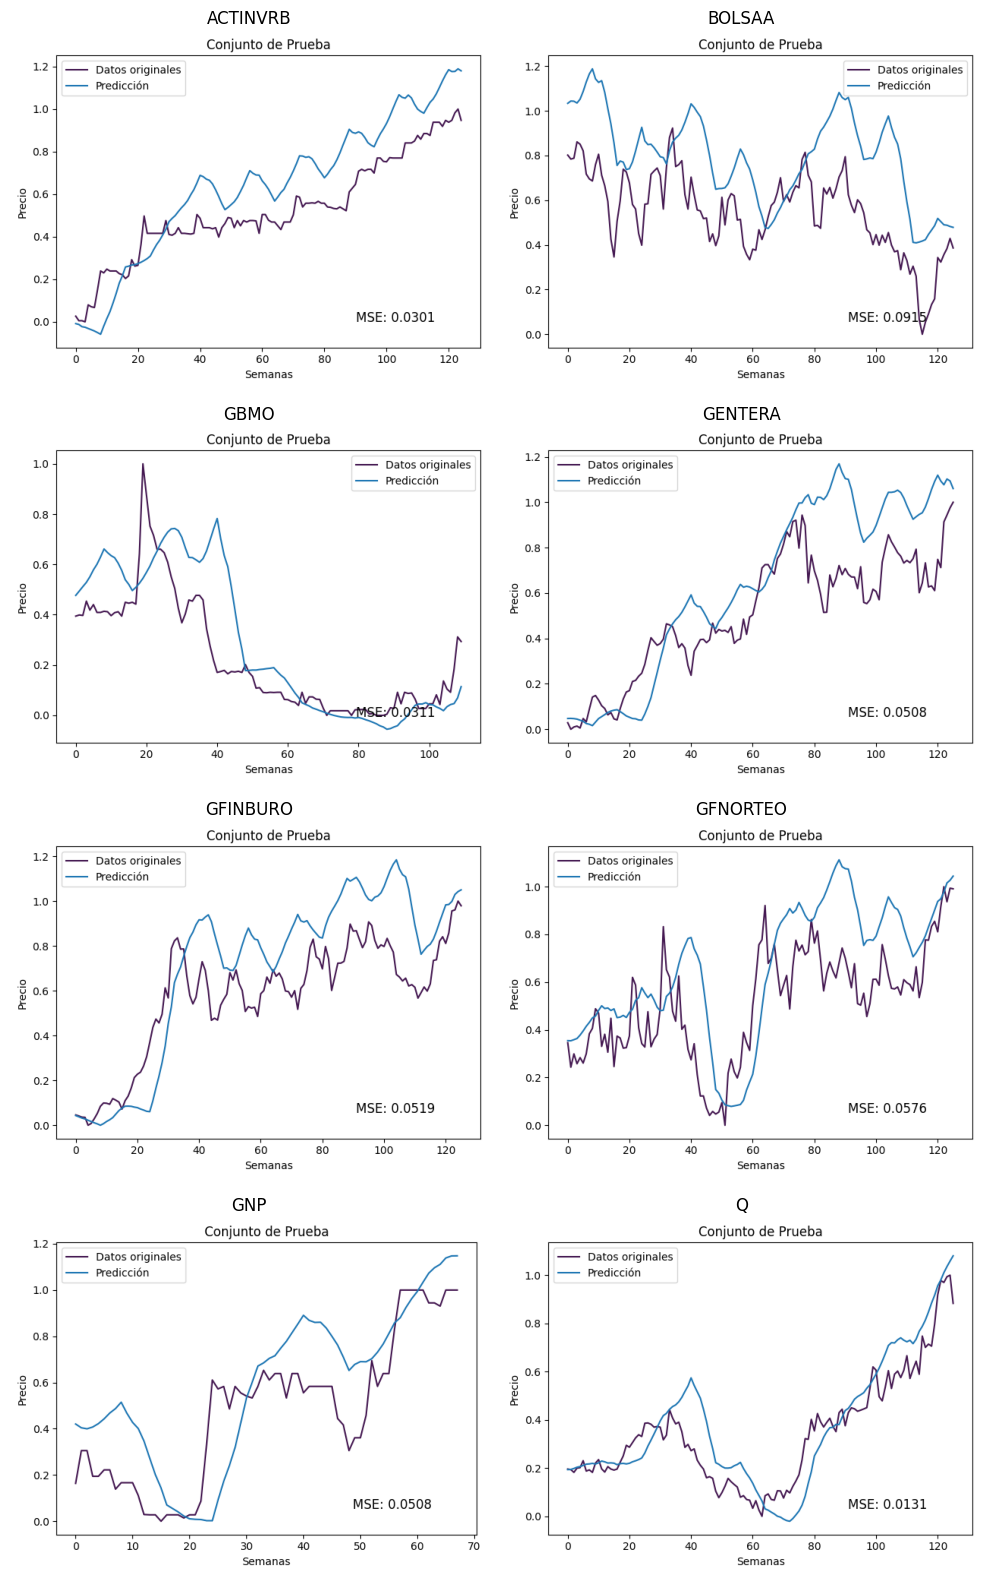
\includegraphics[width=0.8\textwidth]{Figuras/analisis/NARNN.png}
    \caption{Desempeño del modelo NARNN} 
    \label{fig:desempenio_NARNN}
\end{figure}

\begin{figure}[H]
    \centering
    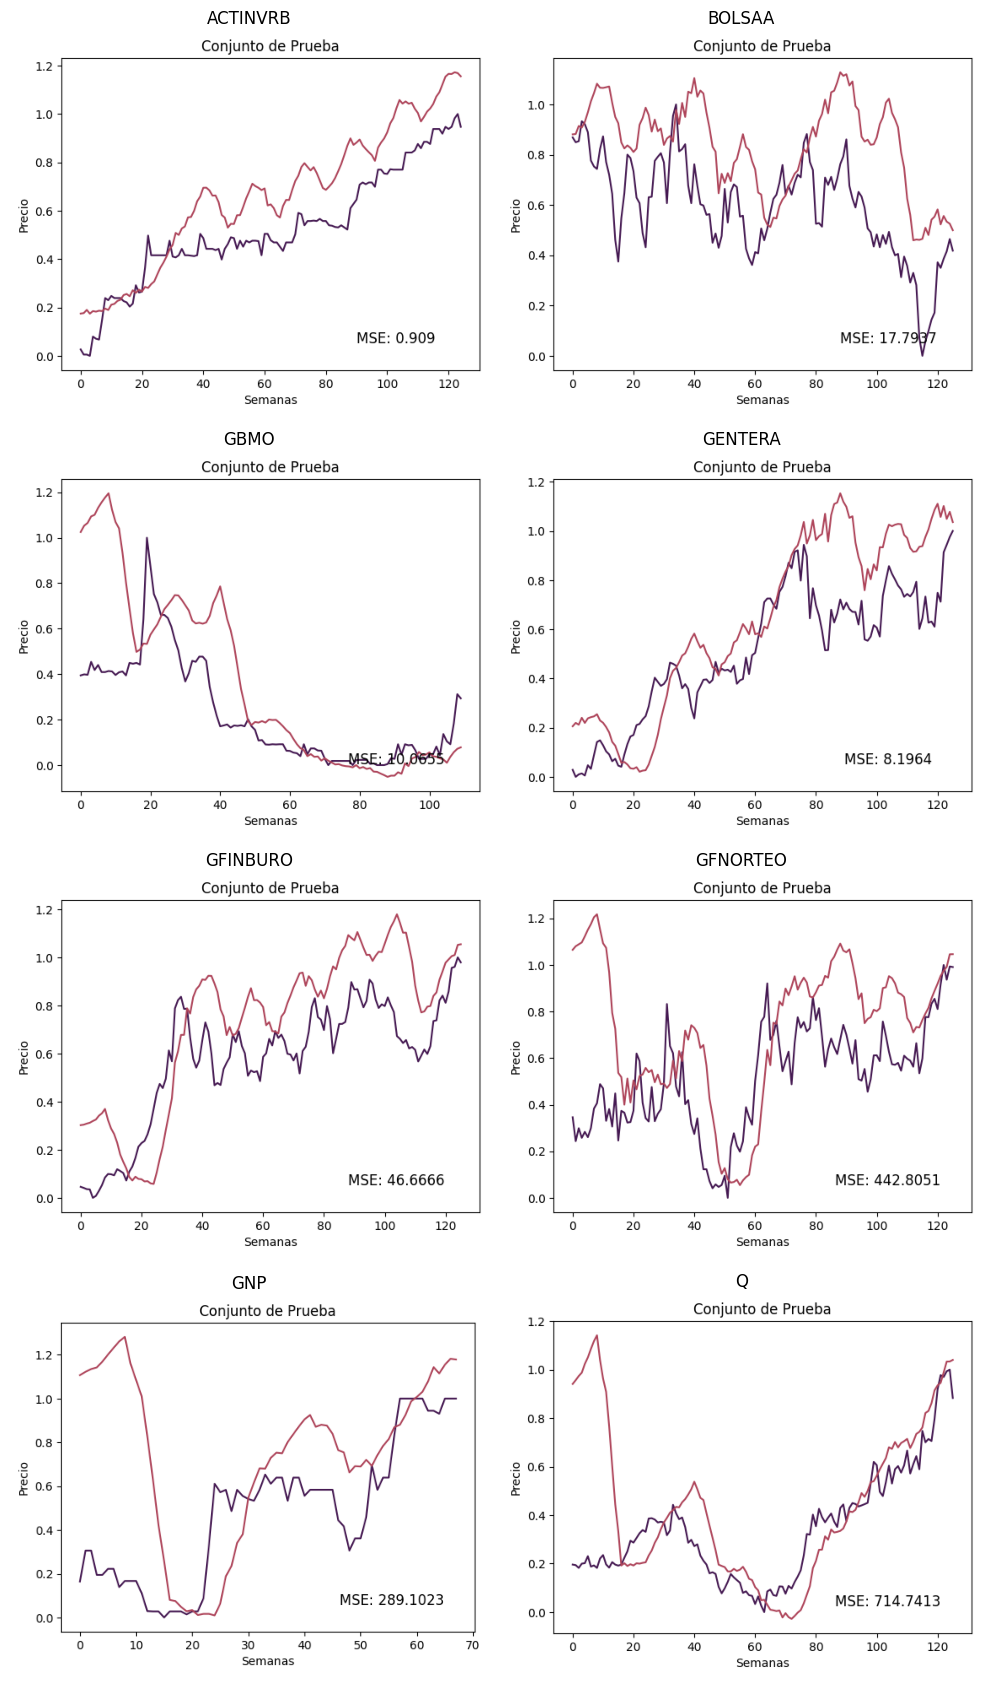
\includegraphics[width=0.8\textwidth]{Figuras/analisis/DWT_NARNN.png}
    \caption{Desempeño del modelo DWT-NARNN} 
    \label{fig:desempenio_DWTNARNN}
\end{figure}

\begin{figure}[H]
    \centering
    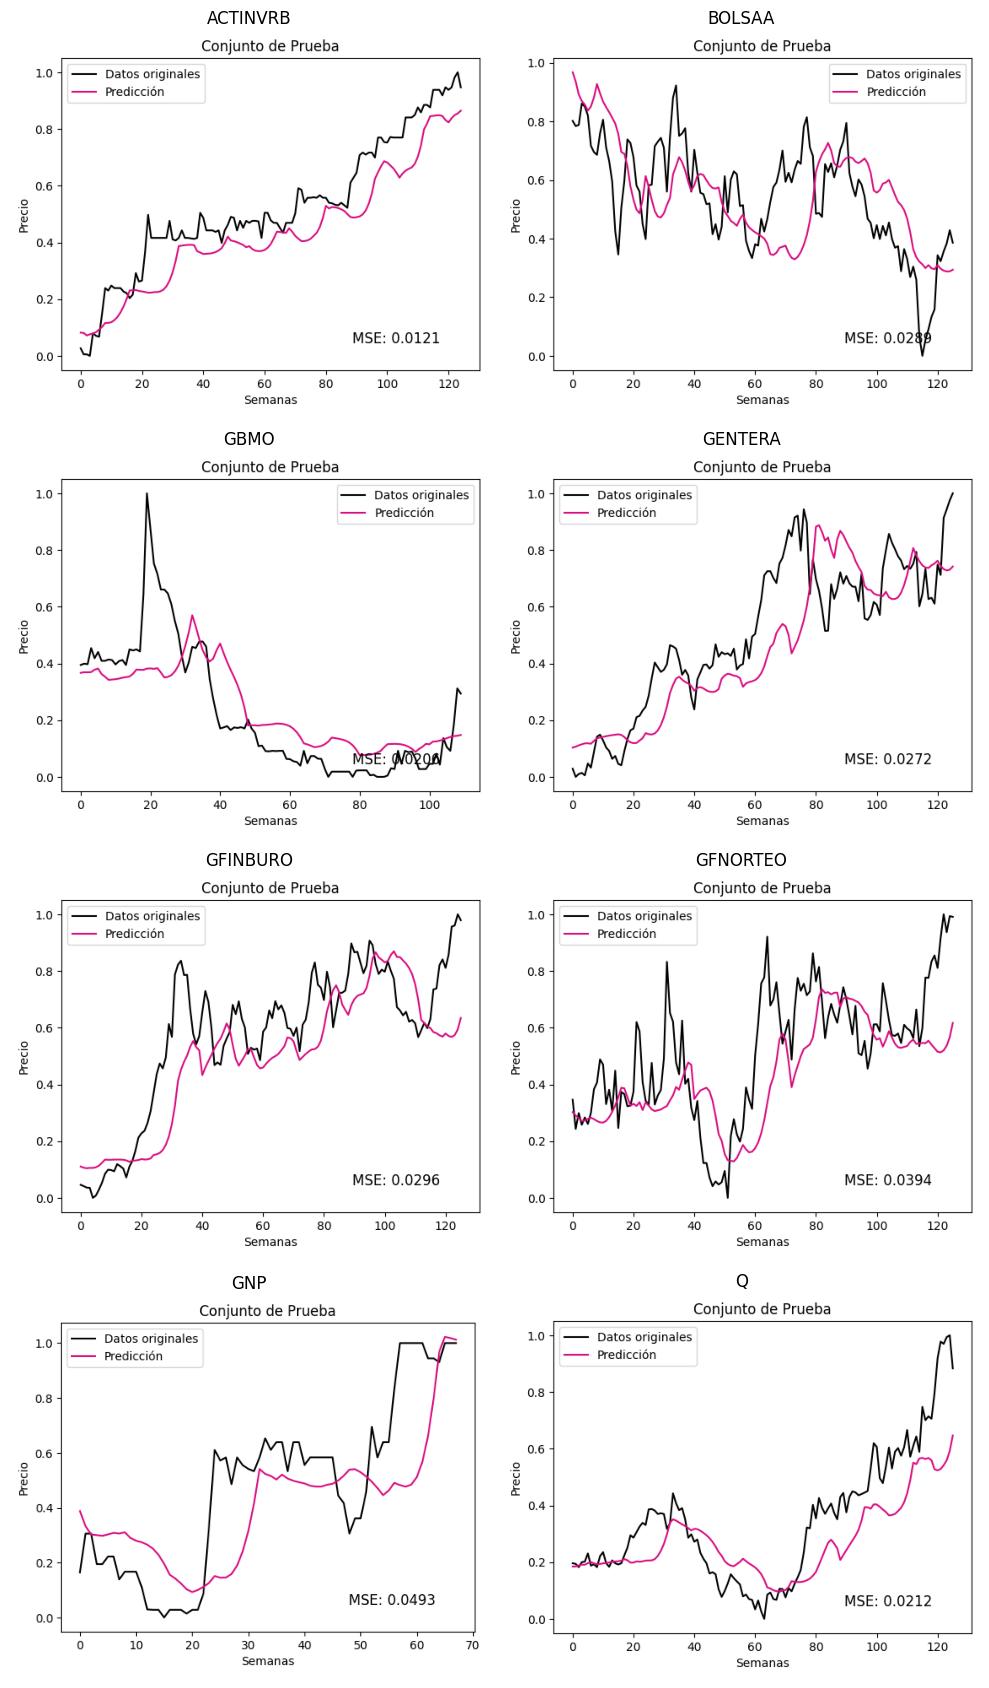
\includegraphics[width=0.8\textwidth]{Figuras/analisis/LSTM.png}
    \caption{Desempeño del modelo LSTM} 
    \label{fig:desempenio_LSTM}
\end{figure}

\begin{figure}[H]
    \centering
    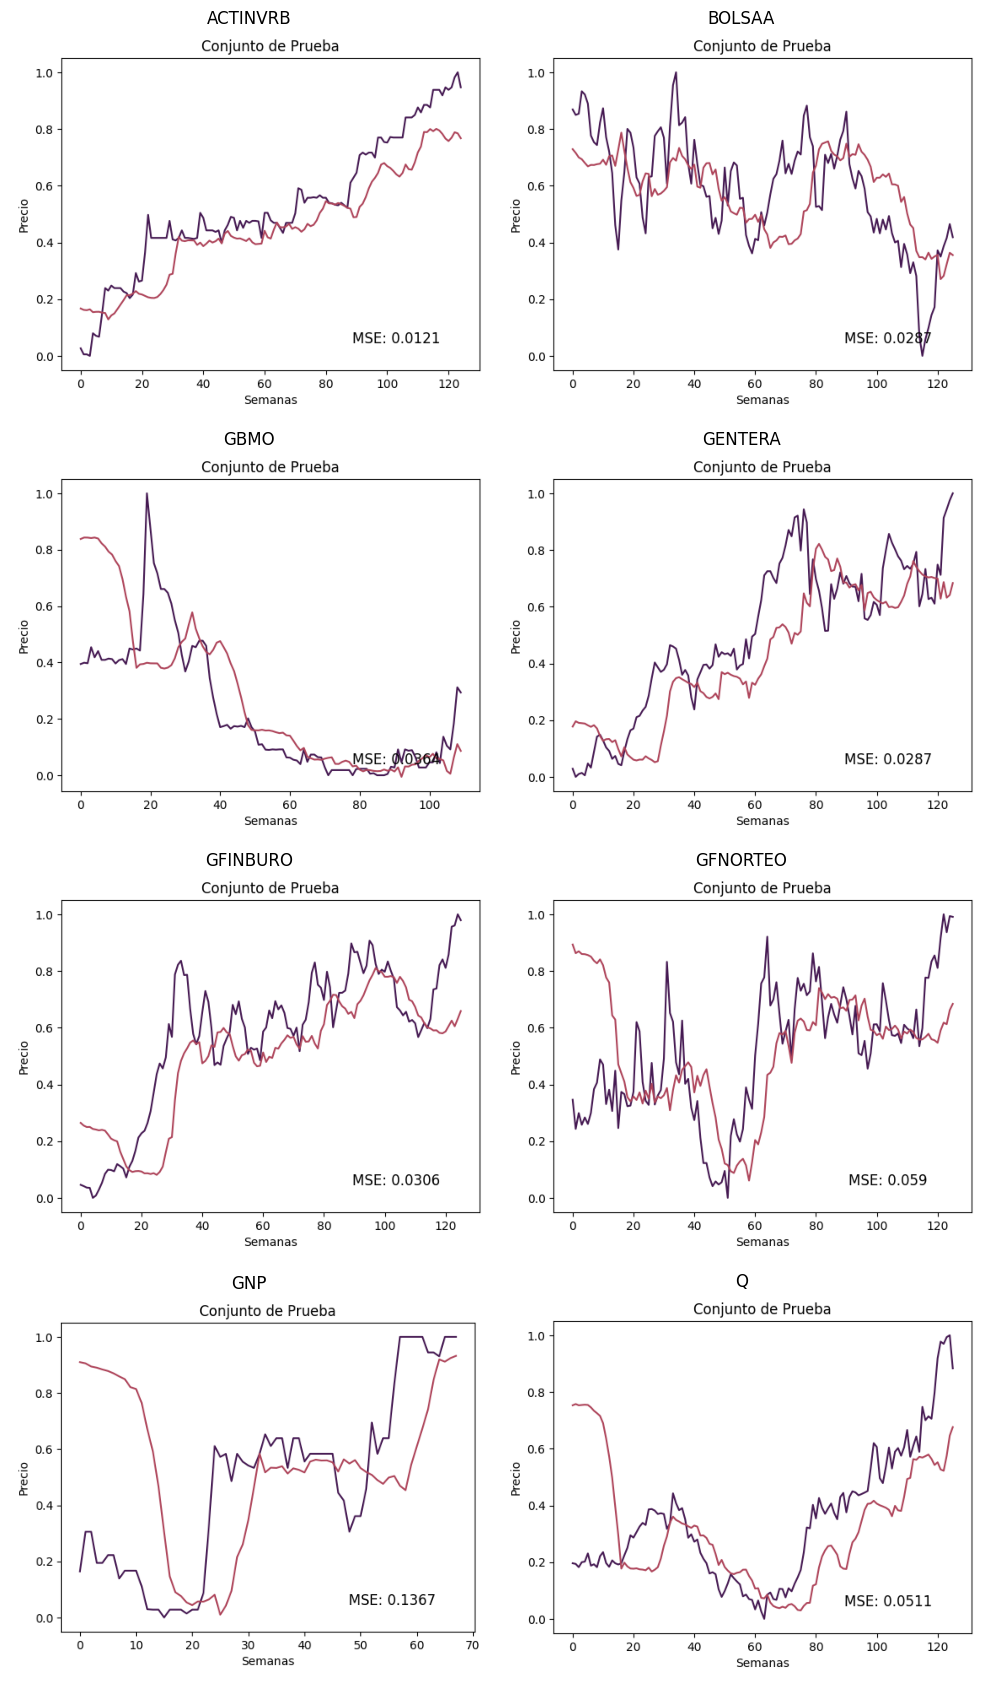
\includegraphics[width=0.8\textwidth]{Figuras/analisis/DWT_LSTM.png}
    \caption{Desempeño del modelo DWT-LSTM} 
    \label{fig:desempenio_DWTLSTM}
\end{figure}

\begin{figure}[H]
    \centering
    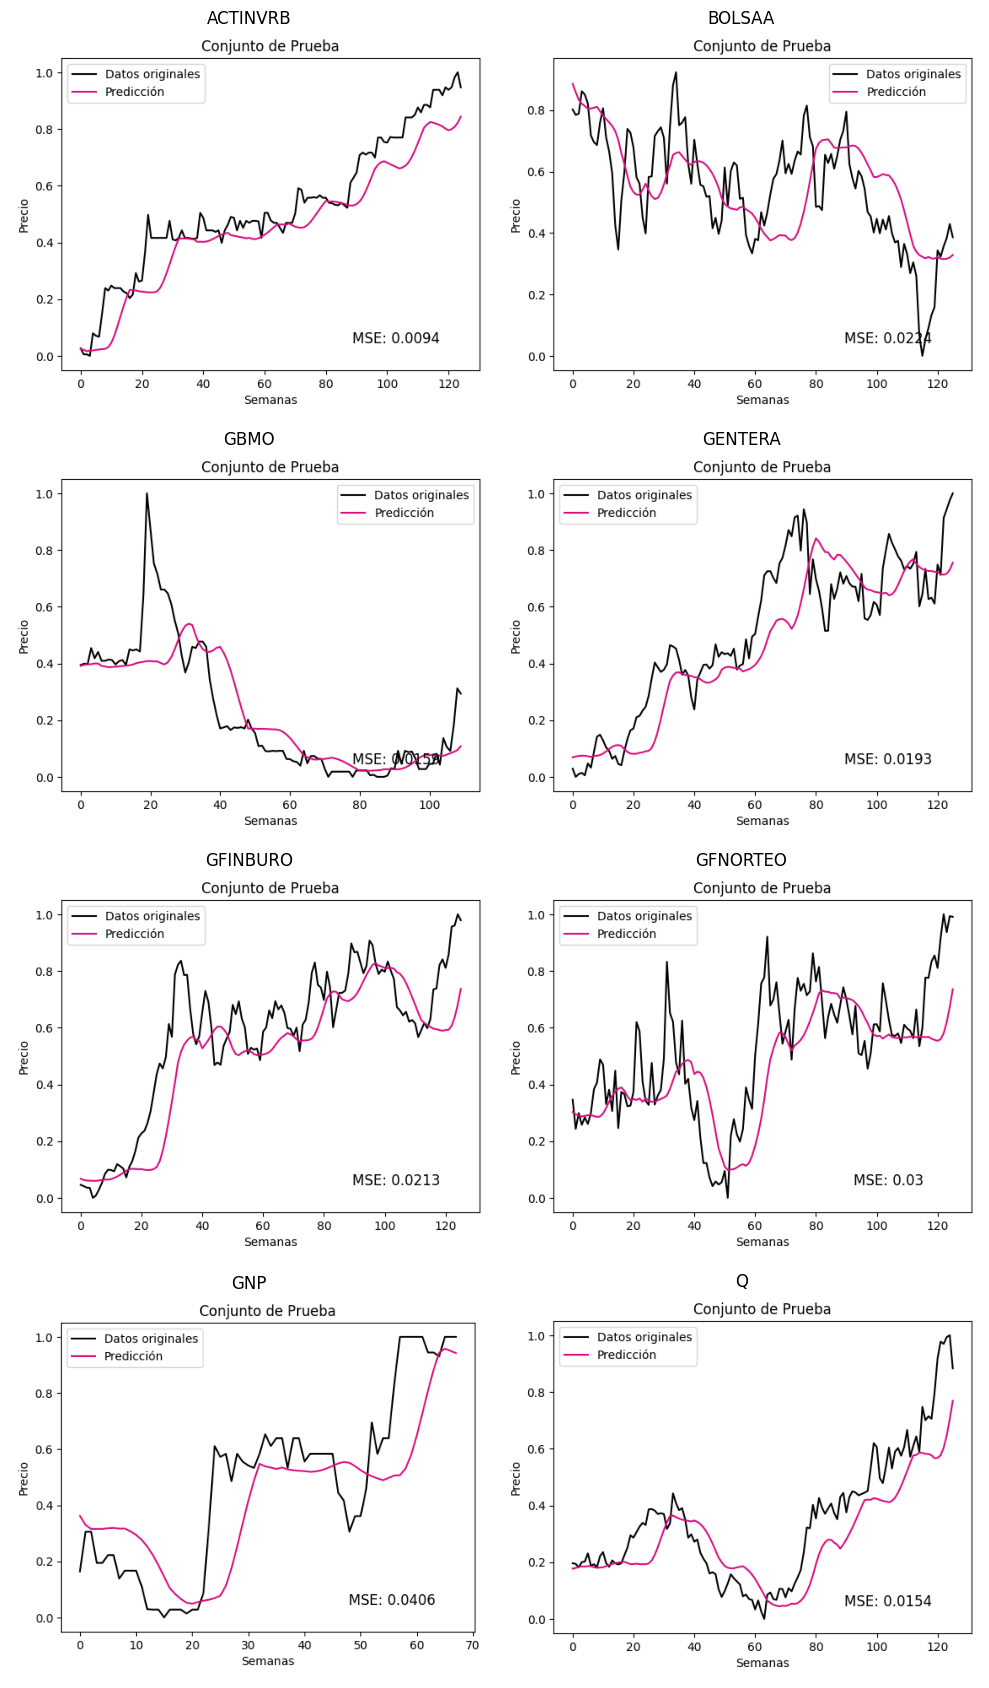
\includegraphics[width=0.8\textwidth]{Figuras/analisis/GRU.png}
    \caption{Desempeño del modelo GRU} 
    \label{fig:desempenio_GRU}
\end{figure}

\begin{figure}[H]
    \centering
    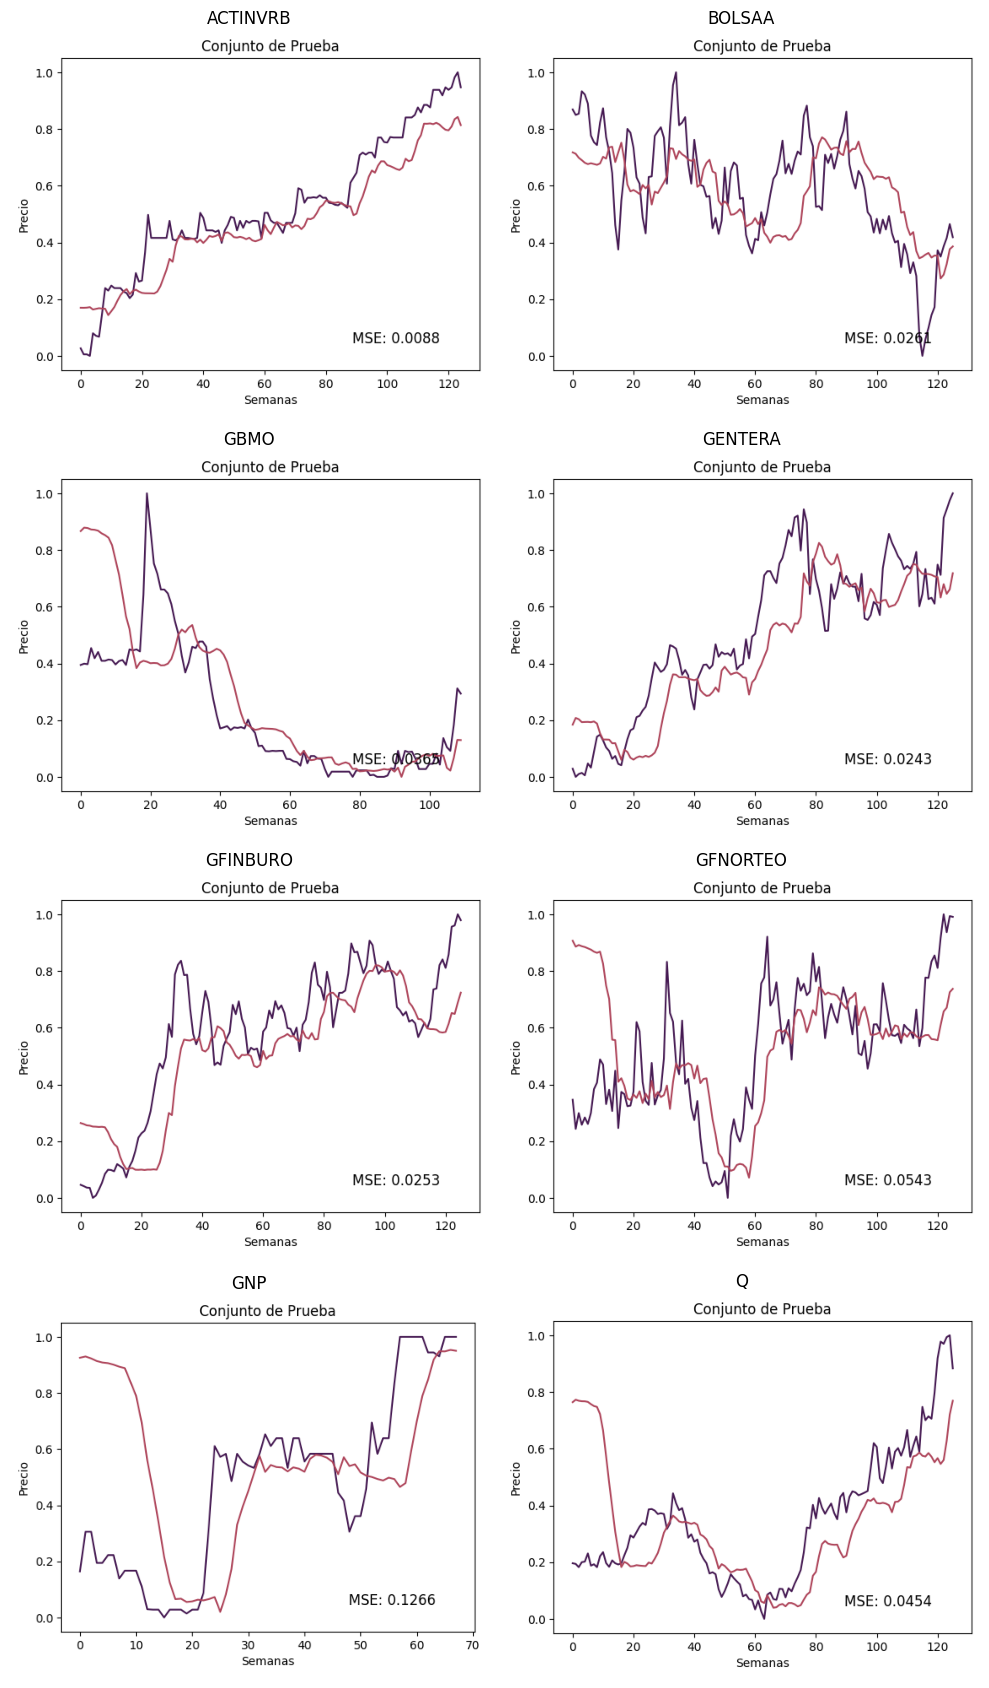
\includegraphics[width=0.8\textwidth]{Figuras/analisis/DWT_GRU.png}
    \caption{Desempeño del modelo DWT-GRU} 
    \label{fig:desempenio_DWTGRU}
\end{figure}

Si se detiene el análisis un momento aquí, se ve en \ref{fig:desempenio_NARNN} y \ref{fig:desempenio_DWTNARNN} que las redes auto-regresivas tienden a sobrestimar los datos (como se ve en ACTINVRB, BOLSAA, GFINBURO y GNP) y a depender mucho de la 'correción' que ofrece este esquema híbrido cada ocho semanas. Vemos como las predicciones en ciertos puntos se alejan bastante de los valores reales y regresan abruptamente en intervalos de ocho semanas, formando estas estructuras con forma de cresta o pico cada cierto tiempo. Formas que no necesariamente son parte del comportamiento original de los datos.

Como se ve en \ref{fig:desempenio_DWTLSTM}, DWT-LSTM mejora la calidad de la predicción respecto a LSTM en \ref{fig:desempenio_LSTM}. La 'correción' que acurre cada ocho semanas se hace menos notoria, ya que los modelos mantienen su buen pronostico por más tiempo. Y en general la señal capta mejor la dirección que tomarán los precios. Ocurre algo similar en \ref{fig:desempenio_DWTGRU} y \ref{fig:desempenio_GRU} correspondientemente. Se observa que para las redes recurrentes es mucho más fácil captar las tendencias de la serie original, y con ayuda de la DWT permiten generar un resultado más cercano a este.

%%%%%%%%%%%%%%%%%%%%%%%%%%%%%%%%%%%%%%%%%%%%%%%%%%%%%%%%%%
%%%%%%%%%%%%%%%%%%%%%%%%%%%%%%%%%%%%%%%%%%%%%%%%%%%%%%%%%%

\subsection{Prueba de Kolmogorov-Smirnov}

Una métrica útil para comparar el desempeño de los modelos es la prueba estadística de Kolmogorov-Smirnov. Esta se enfoca en encontrar la diferencia máxima que existe entre dos distribuciones y así determinar si difieren significativamente entre si. Ya que no requiere asumir que los datos sigan una distribución específica, es sensible a las diferencias en las formas, como la posición, la dispersión y la forma general. Se puede valer de ella como menciona Hassani, H. y Silva, E \cite{kolmogorov}. En este caso se emplea para comparar la distribución de los errores (MSE) de las predicciones de cada modelo y de cada una se obtiene el estadístico $KS$ y el valor $p$. 

Como se observa en las figuras  \ref{fig:DWTNARNN_NARNN}, \ref{fig:DWTLSTM_LSTM}, \ref{fig:DWTGRU_GRU}, los estadísticos y valores $p$ son generados por la prueba bilateral y unilateral (medidas que se ven en el extremo inferior izquierdo de cada imagen). Para saber si existe una diferencia estadísticamente significativa el valor $p$ debe de ser menor a 0.05 en la prueba bilateral, así se rechaza la hipótesis nula y se acepta la alternativa. Y si la segunda distribución reporta un menor error estocástico debe de presentarse el mismo caso que en su homologa anterior pero en la prueba unilateral. 

Dicho lo anterior, Se obtuvo lo siguiente:

\begin{figure}[H]
    \centering
    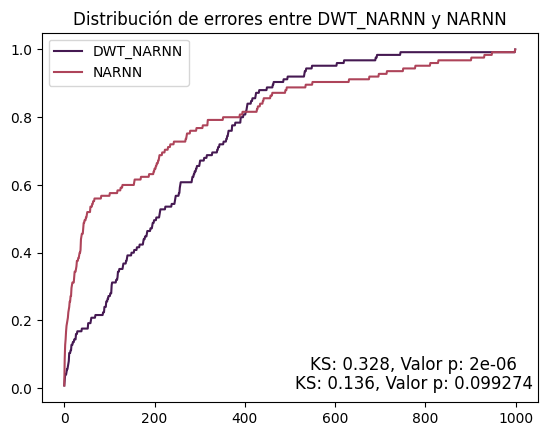
\includegraphics[width=0.5\textwidth]{Figuras/analisis/kolmogorov/DWTNARNN_NARNN.png}
    \caption{Distribución de errores de predicción de los modelos DWT-NARNN vs. NARNN.} 
    \label{fig:DWTNARNN_NARNN}
\end{figure}

Se rechaza la hipótesis nula de la prueba bilateral y se acepta la alternativa ($2e-06 < 0.05$). Los errores no comparten la misma distribución, existe una diferencia estadísticamente significativa. Se acepta la hipótesis nula de la prueba unilateral ($0.0992 > 0.05$), el modelo NARNN reporta un menor error estocástico.

\begin{figure}[H]
    \centering
    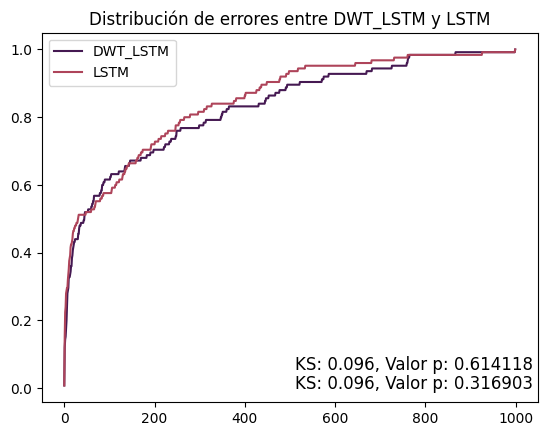
\includegraphics[width=0.5\textwidth]{Figuras/analisis/kolmogorov/DWTLSTM_LSTM.png}
    \caption{Distribución de errores de predicción de los modelos DWT-LSTM vs. LSTM.} 
    \label{fig:DWTLSTM_LSTM}
\end{figure}

Se rechaza la hipótesis nula de la prueba bilateral y se acepta la alternativa ($0.6141 > 0.05$). Los errores no comparten la misma distribución, existe una diferencia estadísticamente significativa. 
Se acepta la hipótesis nula de la prueba unilateral ($0.3169 > 0.05$). el modelo DWT-LSTM reporta un menor error estocástico, debido a la prueba anterior, esta diferencia es mínima.

\begin{figure}[H]
    \centering
    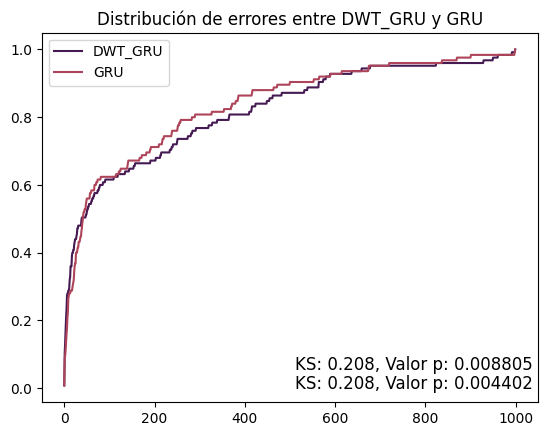
\includegraphics[width=0.5\textwidth]{Figuras/analisis/kolmogorov/DWTGRU_GRU.png}
    \caption{Distribución de errores de predicción de los modelos DWT-GRU vs. GRU.} 
    \label{fig:DWTGRU_GRU}
\end{figure}

Se rechaza la hipótesis nula de la prueba bilateral y se acepta la alternativa ($0.0088 < 0.05$). Los errores no comparten la misma distribución, existe una diferencia estadísticamente significativa. Se rechaza la hipótesis nula de la prueba unilateral y se acepta la alternativa ($0.0044 < 0.05$). El modelo DWT-GRU reporta un menor error estocástico.

Como se ve, los modelos con menor error estocástico son NARNN, DWT-LSTM y DWT-GRU. A continuación en las figuras \ref{fig:NARNN_DWTGRU}, \ref{fig:NARNN_DWTLSTM} se muestra una comparativa entre los tres.

\begin{figure}[H]
    \centering
    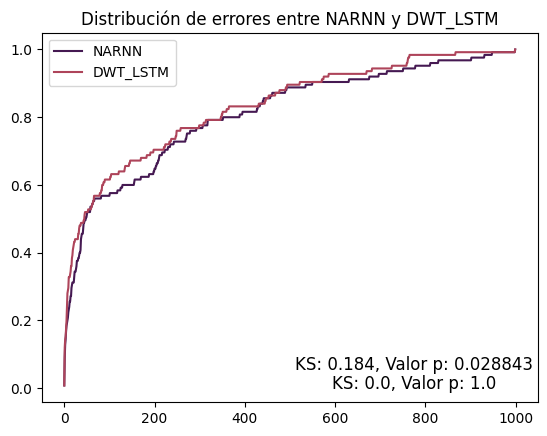
\includegraphics[width=0.5\textwidth]{Figuras/analisis/kolmogorov/NARNN_DWTLSTM.png}
    \caption{Distribución de errores de predicción de los modelos NARNN vs. DWT-LSTM: El modelo DWT-LSTM reporta un menor error estocástico.} 
    \label{fig:NARNN_DWTLSTM}
\end{figure}

\begin{figure}[H]
    \centering
    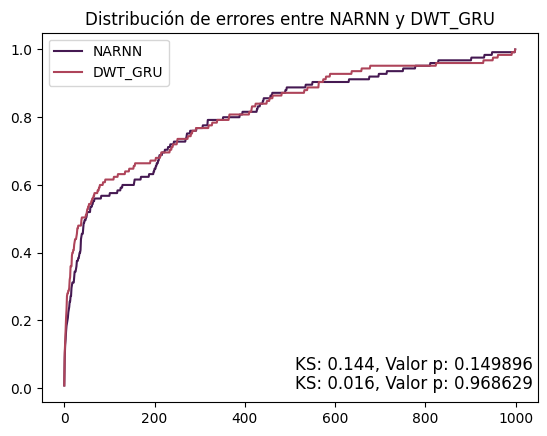
\includegraphics[width=0.5\textwidth]{Figuras/analisis/kolmogorov/NARNN_DWTGRU.png}
    \caption{Distribución de errores de predicción de los modelos NARNN vs. DWT-GRU: El modelo DWT-GRU reporta un menor error estocástico.} 
    \label{fig:NARNN_DWTGRU}
\end{figure}

\begin{figure}[H]
    \centering
    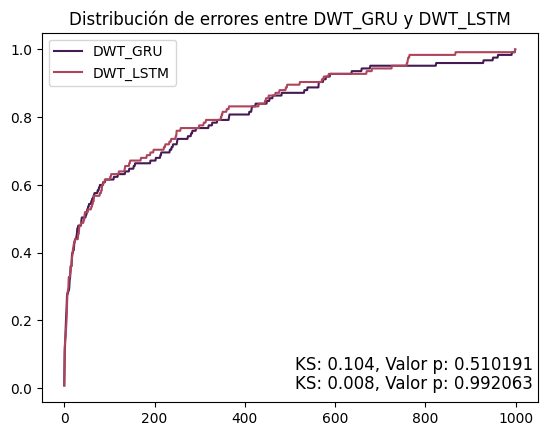
\includegraphics[width=0.5\textwidth]{Figuras/analisis/kolmogorov/DWTGRU_DWTLSTM.png}
    \caption{Distribución de errores de predicción de los modelos DWT-GRU vs. DWT-LSTM: El modelo DWT-LSTM reporta un menor error estocástico.} 
    \label{fig:DWTGRU_DWTLSTM}
\end{figure}

Así, el modelo que muestra un menor error durante la prueba es el DWT-LSTM, un modelo recurrente con descomposición por ondículas.
\newpage
\subsection{Resultados finales}

%%%%%%%%%%%%%%%%%%%%%%%%%%%%%%%%%%%%%%%%%%%%%%%

\begin{figure}[H]
    \centering
    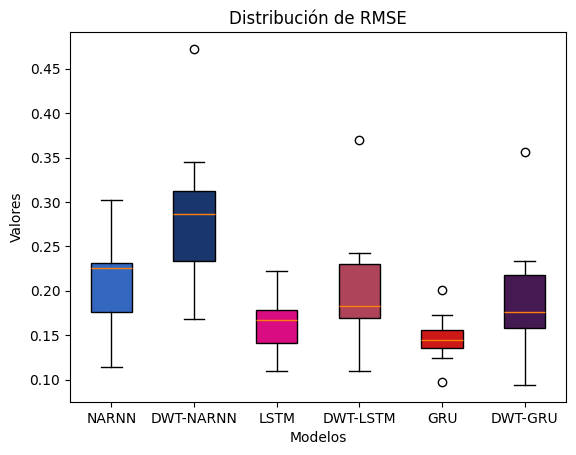
\includegraphics[width=0.6\textwidth]{Figuras/analisis/RMSE.png}
    \caption{Diagrama de caja para métrica RMSE de las predicciones de todos los conjuntos de datos.} 
    \label{fig:RMSE}
\end{figure}

\begin{figure}[H]
    \centering
    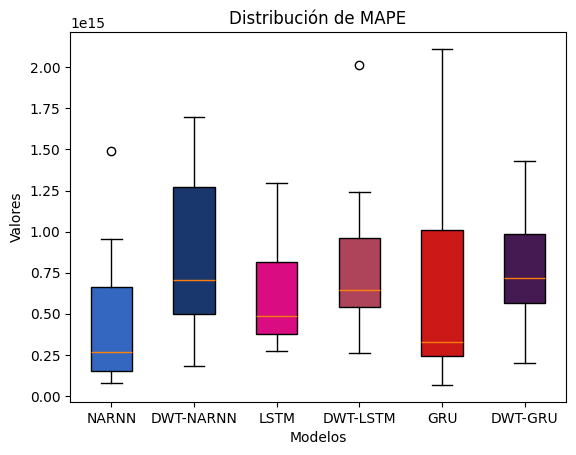
\includegraphics[width=0.6\textwidth]{Figuras/analisis/MAPE.png}
    \caption{Diagrama de caja para métrica MAPE de las predicciones de todos los conjuntos de datos.} 
    \label{fig:MAPE}
\end{figure}

\begin{figure}[H]
    \centering
    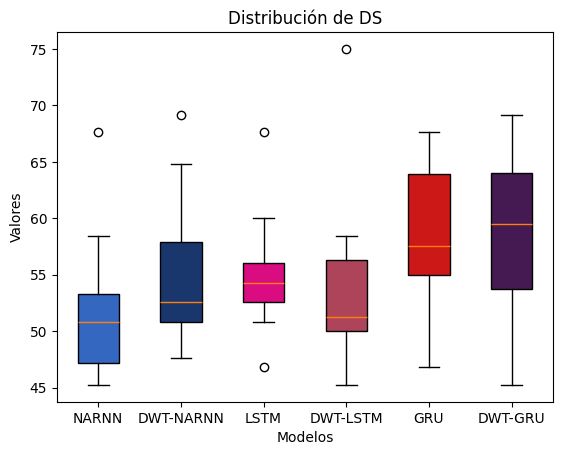
\includegraphics[width=0.6\textwidth]{Figuras/analisis/DS.png}
    \caption{Diagrama de caja para métrica DS de las predicciones de todos los conjuntos de datos.} 
    \label{fig:DS}
\end{figure}

Se organizan los resultados de las métricas durante los tres tipos diferentes de predicción. En el diagrama RMSE, las RNNs ya sea con DWT o no tienen un mejor desempeño de predicción que las NARNNs, un resultado que se esperaba ante el hecho de que las RNNs están capacitadas especialmente para resolver problemas de datos con dependencias a largo plazo como vimos en durante el estudio de redes neuronales.

Es importante destacar que a pesar de que la DWT sea una herramienta fundamentan en el desempeño de una red neuronal, la arquitectura y métodos de entrenamiento de esta son igualmente importantes. Como vimos a lo largo del estudio, la combinación de un pre-procesamiento de datos con una red recurrente nos brinda mejores resultados:

\begin{itemize}
    \item Podemos ver en el diagrama de cajón de RMSE que esta distribución es mayor cuando se usa la DWT (se equivoca más), pero es precisamente debido a la predicción de 'ruido' adicional en la serie, es decir, que al emplear la descomposición y la respectiva predicción en cada una de sus componentes y la posterior recomposición aumenta el ruido en esta y así consecuentemente el error o diferencia entre la serie original y esta. Hecho que no necesariamente significa que la predicción con DWT sea menor acertada, al contrario, la tendencia se ve mejor reflejada como podemos ver con el diagrama de DS.
    \item Los resultados de la predicción respecto a la dirección se adecuan más cuando existe la descomposición a diferencia de las redes que no cuentan con ella, es decir que cuando se usa la DWT, las tendencias de pérdida o ganancia son mejor captadas. Véase que los modelos con mejor desempeño con respecto a esta métrica son el par de GRUnns.
   
\end{itemize}